%!TEX root=../document.tex

\section{Ergebnisse}
\label{sec:Ergebnisse}
\subsection{Tutorial}
Zu Beginn habe ich das Tutorial mit Jersey und JAX-RS umgesetzt, um eine Basiskonfiguration zu erhalte, auf die ich aufbauen kann. Folgende Schritte waren notwendig:
\subsubsection{Programm erstellen}
Zuerst erstellt man ein 'Dynamic Web Project'. Dabei wählt man als Target Runtime Apache Tomcat v9.0. Da bei der Erstellung des Projekts kein web.xml File vorhanden war, habe ich einen Deployment Descriptor Stup generieren lassen.

\begin{figure}[htbp] 
  \centering
     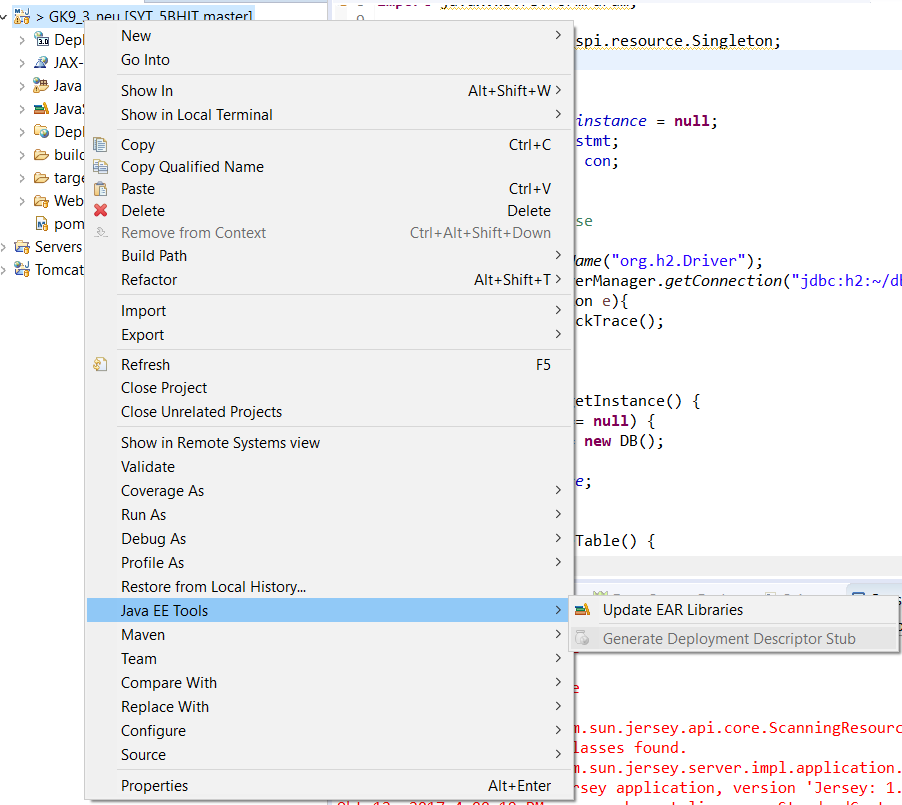
\includegraphics[width=0.7\textwidth]{D:/Schule/5.Jahrgang/SYT/SYT_5BHIT/Protokoll/latex_template/images/schritt1.PNG}
  \caption{Generate Deployment Descriptor Stup}
  \label{fig:Bild1}
\end{figure}

\subsubsection{pom.xml}
Nun konvertiert man das Projekt in ein Maven-Project und added folgende Dependencies in das pom.xml File:
\begin{itemize}
	\item asm.jar
	\item jersey-bundle.jar
	\item json.jar
	\item jersey-server.jar
\end{itemize}

Hier ein Auschschnitt wie man eine Dependencie in ein pom.xml hinzufügt.
\begin{figure}[htbp] 
  \centering
     \includegraphics[width=0.7\textwidth]{D:/Schule/5.Jahrgang/SYT/SYT_5BHIT/Protokoll/latex_template/images/schritt2.PNG}
  \caption{Dependency-Struktur in pom.xml}
  \label{fig:Bild1}
\end{figure}

\subsection{Register}
Beim Register habe ich als Path /register gemäß der Aufgabenstellung angegeben.
\begin{figure}[htbp] 
  \centering
     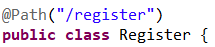
\includegraphics[width=0.7\textwidth]{D:/Schule/5.Jahrgang/SYT/SYT_5BHIT/Protokoll/latex_template/images/schritt3.PNG}
  \caption{Path von Register}
  \label{fig:Bild1}
\end{figure}

\subsubsection{register() Methode}
In der Klasse habe ich die Methode register() geschrieben, welche das Registrierungsformular zur Verfügung stellt. Wichtig ist dabei die @Produces Annotation. Diese sagt aus, dass die Methode etwas produziert/darstellt. Der Parameter besagt was genau dabei erstellt wird, in diesem Fall eine HTML-Seite.
 \begin{figure}[htbp] 
  \centering
     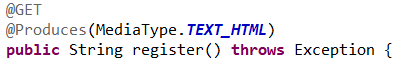
\includegraphics[width=0.7\textwidth]{D:/Schule/5.Jahrgang/SYT/SYT_5BHIT/Protokoll/latex_template/images/schritt4.PNG}
  \caption{Annotations von register()}
  \label{fig:Bild1}
\end{figure}
Die Klasse liefert ein String zurück, indem das HTML für die Seite dabeisteht.
\begin{figure}[htbp] 
  \centering
     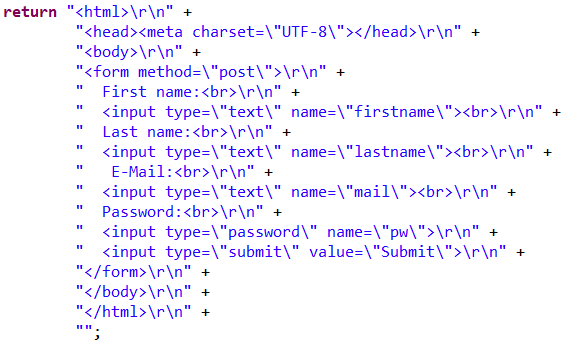
\includegraphics[width=0.5\textwidth]{D:/Schule/5.Jahrgang/SYT/SYT_5BHIT/Protokoll/latex_template/images/schritt5.PNG}
  \caption{HTML von Register}
  \label{fig:Bild1}
\end{figure}

\subsubsection{submit() Methode}
